\subsection{Starting Fresh}
\label{sec:loadSourceMeta}
\begin{itemize}

\item[$\blacktriangleright$] To get started in Eclipse, press the \texttt{Install, configure and deploy Moflon} button and navigate to ``Install Workspace''. Choose ``Handbook Example (Part 4)''. It contains the full \texttt{LeitnersLearningBox} metamodel, as well as each method implemented as an SDM and an example instance in ``LearningBoxLanguage/instances/''.

\begin{figure}[htbp]
\begin{center}
  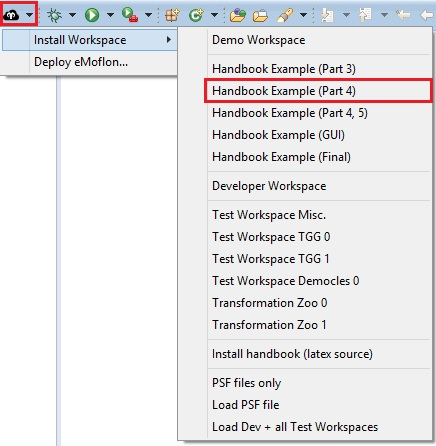
\includegraphics[width=0.65\textwidth]{eclipse_part4FreshWizardDownload}
  \caption{Initialize your workspace with your preferred syntax}
  \label{eclipse:downPartIV}
\end{center}
\end{figure}

\vspace{0.5cm}

\item[$\blacktriangleright$] After loading, if your workspace does not resemble ours in Fig.~\ref{eclipse:workingSets}, with eMoflon's ``Build'' icon on the
tooolbar and a package explorer with at least two distinct nodes, first switch to the eMoflon perspective by navigating to ``Window/Open
Perspective/Other\ldots'' and choosing ``eMoflon'' from the list. Then, select the small downward-facing arrow in the upper right corner of the package
explorer. ``Top Level Elements/Working Sets.'' To review how these nodes are used to structure our workspace in Eclipse, check out Part I, Section 4.

\vspace{0.5cm}

\begin{figure}[htbp]
	\centering
  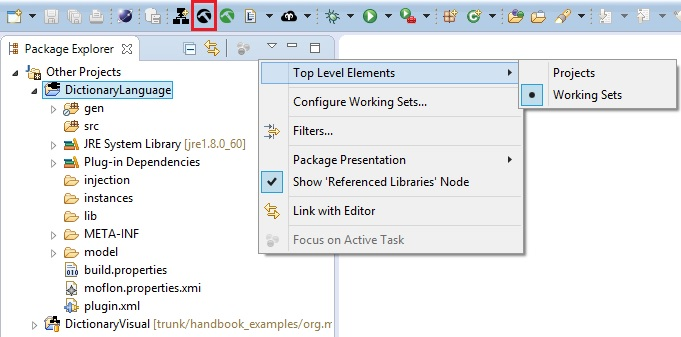
\includegraphics[width=0.9\textwidth]{eclipse_workingSets}
	\caption{Setting your Package Explorer}
	\label{eclipse:workingSets}
\end{figure}

\vspace{0.5cm}

\item[$\blacktriangleright$] Fantastic -- you now have the source metamodel for your transformation ready to go!

\end{itemize}